\documentclass[10pt]{beamer}

\usepackage[brazilian]{babel}
\usepackage[utf8]{inputenc}
\usepackage{graphicx}
\usepackage{mathtools}
\usepackage{amsthm}
\usepackage{thmtools,thm-restate}
\usepackage{amsfonts}
\usepackage{hyperref}
\usepackage[singlelinecheck=false]{caption}
\usepackage[backend=biber,url=true,doi=true,eprint=false,style=alphabetic]{biblatex}
\usepackage[justification=centering]{caption}
\usepackage{indentfirst}
\usepackage{algorithm}
\usepackage{algpseudocode}
\usepackage{listings}

%remove line breaks
\setbeamertemplate{bibliography entry title}{}
\setbeamertemplate{bibliography entry location}{}
\setbeamertemplate{bibliography entry note}{}

\uselanguage{Brazilian}
\languagepath{Brazilian}
\usetheme{Berlin}

\addbibresource{references.bib}

\makeatletter
\def\subsection{\@startsection{subsection}{3}%
  \z@{.5\linespacing\@plus.7\linespacing}{.1\linespacing}%
  {\normalfont\itshape}}
\makeatother

\DeclareMathOperator*{\argmin}{arg\,min}
\DeclareMathOperator*{\argmax}{arg\,max}

\newcommand\defeq{\mathrel{\overset{\makebox[0pt]{\mbox{\normalfont\tiny\sffamily def}}}{=}}}

\algrenewcommand\algorithmicrequire{\textbf{Input}}
\algrenewcommand\algorithmicensure{\textbf{Output}}

\captionsetup[table]{labelsep=space}

\theoremstyle{plain}

\newtheorem{proposition}{Proposição}
\newtheorem{exercise}{Exercício}

\newcommand{\set}[1]{\mathbf{#1}}
\newcommand{\pr}{\mathbb{P}}
\renewcommand{\implies}{\Rightarrow}

\newcommand{\bigo}{\mathcal{O}}
\newcommand{\p}{\pause}

\setlength{\parskip}{1em}

\lstset{frameround=fttt,
  language=[5.3]Lua,
	numbers=left,
	breaklines=true,
	keywordstyle=\bfseries,
	basicstyle=\ttfamily,
}

\newcommand\Fontsmall{\fontsize{12}{7.2}\selectfont}

\newcommand{\code}[1]{\lstinline[mathescape=true]{#1}}
\newcommand{\mcode}[1]{\lstinline[mathescape]!#1!}

\title{Estudo sobre Sum-Product Networks e Aprendizagem Profunda}
\author{Renato Lui Geh}
\institute[IME-USP] {%
  Instituto de Matemática e Estatística\\
  Universidade de São Paulo
}
\titlegraphic{\hspace*{7.5cm}~
\includegraphics[scale=0.25]{imgs/logo.png}}

\begin{document}

\frame{\titlepage}

\begin{frame}
  \frametitle{Índice}
  \tableofcontents
\end{frame}

%--------------------------------------------------------------------------------------------------

\section{Notação}

\begin{frame}
  \frametitle{Notação}
  \begin{tabular}{l@{}l@{}p{3in}}
    $\set{X,Y,x,y}$\hspace*{0.6cm}&:\hspace*{0.2cm}& conjuntos\pause\\
    $\Pr$&: & distribuição ou função de probabilidade\pause\\
    $\set{X}$&: & conjunto de variáveis aleatórias\pause\\
    $\set{x}$&: & instanciação de $\set{X}$ (i.e.\ $\set{X}=\set{x}$)\pause\\
    $Val(X)$&: & domínio de $X$\pause\\
    $G=(V,E)$&: & grafo com vértices $V$ e arestas $E$\pause\\
    $Pa(X)$&: & pais de $X$\pause\\
    $Ch(X)$&: &filhos de $X$\pause\\
    $\bigo$&: & notação assintótica\pause\\
    $\Omega$&: & espaço de possibilidades\pause\\
    $\mathcal{F}$&: & álgebra de conjuntos\\
  \end{tabular}
\end{frame}

%--------------------------------------------------------------------------------------------------

\section{Introdução}

\begin{frame}
  \frametitle{Representação em Inteligência Artificial}
  \begin{itemize}
    \item Logica proposicional e de primeira ordem\p
      \begin{itemize}
        \item Todo homem é mortal\p
        \item Sócrates é homem\p
        \item Sócrates é mortal\p
      \end{itemize}
    \item Lógica difusa\p
      \begin{itemize}
        \item 2.0 m é 0.8 alto\p
        \item 2.5 m é 0.9 alto\p
      \end{itemize}
    \item Probabilidade
  \end{itemize}
\end{frame}

\begin{frame}
  \frametitle{Probabilidade em Inteligência Artificial}

  \begin{itemize}
    \item Lógica proposicional
      \begin{itemize}
        \item Toda ave voa.\p
      \end{itemize}
    \item Lógica difusa
      \begin{itemize}
        \item Sabiá é mais ave?
        \item Avestruz é menos ave?\p
      \end{itemize}
    \item Probabilidade
      \begin{itemize}
        \item $\Pr(Voar=1|Ave=1)=0.8$
        \item $\Pr(Voar=0|Ave=1)=0.2$
      \end{itemize}
  \end{itemize}
\end{frame}

%--------------------------------------------------------------------------------------------------

\section{Motivação}
\begingroup
\tiny
\begin{frame}
  \frametitle{Complexidade de distribuições}

  \begin{example}
    \textbf{Dado de 6 faces não viesado:}

    $X$ se o número da face é par\\
    $Y$ se o número da face é múltiplo de três

    \begin{table}[h]
      \begin{center}
        \begin{tabular}{c | c c | r}
          $\set{x}$ & $X$ & $Y$ & $\Pr(x, y)$ \\
          \hline
          $\{x=1,y=1\}$ & $1$ & $1$ & $1/6$ \\
          $\{x=1,y=0\}$ & $1$ & $0$ & $1/2$ \\
          $\{x=0,y=1\}$ & $0$ & $1$ & $2/6$ \\
          $\{x=0,y=0\}$ & $0$ & $0$ & $1/6$ \\
        \end{tabular}
        \captionsetup{font=scriptsize}
        \caption*{\scriptsize O número de termos desta distribuição é $2^2$.}
      \end{center}
    \end{table}

    Complexidade: $\bigo((\max_i |Val(X_i)|)^n)$
  \end{example}
\end{frame}
\endgroup

%--------------------------------------------------------------------------------------------------

\section[PGMs]{Modelos Probabilísticos Baseados em Grafo}

\begin{frame}
  \frametitle{Modelos Probabilísticos Baseados em Grafo (PGMs)}

  \begin{enumerate}
    \item Modelos:
      \begin{itemize}
        \item Redes Bayesianas (Bayesian Networks)
        \item Redes de Markov (Markov Random Fields)
        \item Grafos de potenciais (Factor Graphs)
        \item Máquinas de Boltzmann (Restricted Boltzmann Machine)
        \item Redes Soma-Produto (Sum-Product Networks)\p
      \end{itemize}
    \item Aplicação:
      \begin{itemize}
        \item Reconhecimento de voz
        \item Processamento de imagens
        \item Multi-classificação
        \item Diagnose médica
        \item Predição de interação de genes e proteínas
        \item Entre outros
      \end{itemize}
  \end{enumerate}
\end{frame}

\begin{frame}
  \frametitle{Redes Bayesianas}
  \begin{definition}
    Uma Rede Bayesiana $\mathcal{N}$ é uma tupla $\mathcal{N}=(\Omega,\mathcal{F},\Pr,G)$, onde
    $\Omega$ é o espaço de possibilidades, $\mathcal{F}$ é uma álgebra sobre $\Omega$, $\Pr$ é uma
    função de probabilidade e $G=(\set{X},E)$ é um grafo onde $\set{X}$ é o conjunto de variáveis de
    $\mathcal{N}$ e $E$ é o conjunto de arestas. Cada variável aleatória $X_i\in\set{X}$ representa
    uma probabilidade condicional $\Pr(X_i|Pa(X_i))$. Uma Rede Bayesiana é uma representação para a
    distribuição de probabilidade conjunta

    \begin{equation}\label{factorization-thm}
      \Pr(\set{X}=\{X_1,\ldots,X_n\})=\prod_{X\in\set{X}} \Pr(X|Pa(X)).
    \end{equation}
  \end{definition}
\end{frame}

\begingroup
\tiny
\begin{frame}
  \frametitle{Redes Bayesianas}
  \begin{figure}[h]
    \centering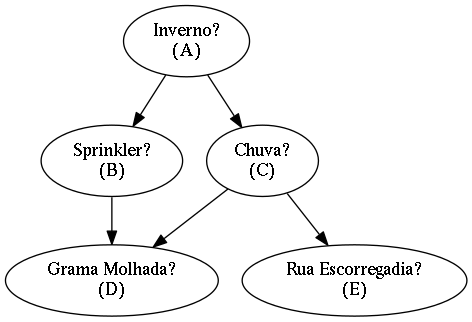
\includegraphics[scale=0.25]{imgs/bn.png}
  \end{figure}

  \begin{table}[h]
    \begin{center}
      \begin{tabular}{l | l}
        $A$ & $\Theta_A$\\
        \hline
        true & $.6$ \\
        false & $.4$ \\
      \end{tabular}
      \begin{tabular}{l l | l}
        $A$ & $B$ & $\Theta_{B|A}$\\
        \hline
        true & true & $.2$ \\
        true & false & $.8$ \\
        false & true & $.75$ \\
        false & false & $.25$ \\
      \end{tabular}
      \begin{tabular}{l l | l}
        $A$ & $C$ & $\Theta_{C|A}$ \\
        \hline
        true & true & $.8$ \\
        true & false & $.2$ \\
        false & true & $.1$ \\
        false & false & $.9$ \\
      \end{tabular}
      \begin{tabular}{l l l | l}
        $B$ & $C$ & $D$ & $\Theta_{D|B,C}$ \\
        \hline
        true & true & true & $.95$ \\
        true & true & false & $.05$ \\
        true & false & true & $.9$ \\
        true & false & false & $.1$ \\
        false & true & true & $.8$ \\
        false & true & false & $.2$ \\
        false & false & true & $0$ \\
        false & false & false & $1$ \\
      \end{tabular}
      \begin{tabular}{l l | l}
        $C$ & $E$ & $\Theta_{E|C}$ \\
        \hline
        true & true & $.7$ \\
        true & false & $.3$ \\
        false & true & $0$ \\
        false & false & $1$ \\
      \end{tabular}
    \end{center}
  \end{table}
\end{frame}
\endgroup

\begingroup
\scriptsize
\begin{frame}
  \frametitle{Inferência Exata em RBs}

  Seja $\set{Y}\subset\set{X}$.
  \begin{align*}
    &\Pr(\set{X})=\prod_{X\in\set{X}} \Pr(X|Pa(X))\\
    &\Pr(\set{Y})=\sum_{X\in\set{X}\setminus\set{Y}} \Pr(X, \set{Y})\\
  \end{align*}
  No nosso exemplo:
  \begin{equation*}
    \Pr(A,B,C,D,E)=\Pr(A)\Pr(B|A)\Pr(C|A)\Pr(D|B,C)\Pr(E|C)
  \end{equation*}
  Probabilidade condicional:
  \begin{equation*}
    \Pr(\set{X}|\set{E})=\frac{\Pr(\set{X},\set{E})}{\Pr(\set{E})}
  \end{equation*}
\end{frame}
\endgroup

\begin{frame}
  \frametitle{Complexidade da Inferência Exata}

  Complexidade: $\bigo((m+n)c^{\omega+1})$
  \begin{align*}
    m &: \text{tamanho do maior conjunto de tabelas}\\
    n &: \text{número de variáveis}\\
    c &: \max_i |Val(X_i)|\\
    \omega &: \text{maior escopo}\\
  \end{align*}
  Exponencial e portanto intratável.
\end{frame}

\begin{frame}
  \frametitle{NP-completude e SAT}
  Inferência exata é análogo ao problema de NP-completude de SAT\@.\p
  \begin{equation*}
    A\vee(B\wedge(C\vee (D\wedge E\vee F)))\p
  \end{equation*}
  Se inferência exata em RBs for subexponencial, então o problem SAT é subexponencial.\p

  \centering{\textbf{Resolvemos um problema relacionado a P vs NP!~$\ddot\smile$~\cite{np-sat}}}\p

  Portanto, acredita-se que não é possível.~$\ddot\frown$\p

  Solução: inferência aproximada.
\end{frame}

\begin{frame}
  \frametitle{Inferência Aproximada}
  \begin{enumerate}
    \item Amostragem estocástica:
    \begin{itemize}
      \item Lógica;
      \item Por importância de verossimilhança;
      \item Amostragem de Gibbs;
    \end{itemize}
    \item Propagação de crença;
    \item Algoritmo soma-produto;
    \item entre outros.
  \end{enumerate}

  Inferência aproximada $\implies$ aprendizado aproximado.
\end{frame}

%--------------------------------------------------------------------------------------------------

\section[SPNs]{Sum-Product Networks}

\begin{frame}
  \frametitle{Network polynomial}

  \begin{definition}
  O polinômio da rede (\emph{network polynomial}) é a função da soma de todas as instanciações da
  distribuição conjunta de uma Rede Bayesiana multiplicadas com as variáveis indicadoras de cada
  variável.

  \begin{equation*}
    f(\set{X})=\sum_{\set{x}\sim\set{X}} \lambda_{\set{x}}\theta_{\set{x}|v\sim Pa(\set{x})}
  \end{equation*}

  Uma variável indicadora é $1$ se a variável é consistente com a instanciação e 0 caso contrário.
  Caso a variável não seja instanciada, a variável indicadora é $1$.
  \end{definition}
\end{frame}

\begin{frame}
  \frametitle{Network polynomial}

  \begin{figure}[h]
    \centering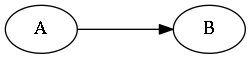
\includegraphics[scale=0.3]{imgs/simple_bn.png}
  \end{figure}

  \begin{table}[h]
    \begin{center}
      \begin{tabular}{l | l}
        $A$ & $\Theta_A$ \\
        \hline
        true & $.7$ \\
        false & $.3$ \\
      \end{tabular}
      \begin{tabular}{l l | l}
        $A$ & $B$ & $\Theta_{B|A}$ \\
        \hline
        true & true & $.2$ \\
        true & false & $.8$ \\
        false & true & $.6$ \\
        false & false & $.4$ \\
      \end{tabular}
    \end{center}
  \end{table}


  \begin{equation*}
    f(A,B)=\lambda_a\lambda_b\theta_a\theta_{b|a}+\lambda_{\overline{a}}\lambda_b
    \theta_{\overline{a}}\theta_{b|\overline{a}}+\lambda_a\lambda_{\overline{b}}\theta_a
    \theta_{\overline{b}|a}+\lambda_{\overline{a}}\lambda_{\overline{b}}
    \theta_{\overline{a}}\theta_{\overline{b}|\overline{a}}
  \end{equation*}
\end{frame}

\begin{frame}
  \frametitle{Sum-Product Networks}
  \begin{definition}
  Uma SPN $S$ é um DAG com três tipos de nós: soma, produto e indicadores. Todo nó indicador é uma
  folha. Todo nó soma tem pais produto, e todo nó produto tem pais soma. Toda aresta com destino a
  um nó soma tem uma aresta com um peso associado. O valor de um nó soma $i$ é $\sum_{j\in Ch(i)}
  w_{ij}v_j$ e o valor de um nó produto $i$ é $\prod_{j\in Ch(i)}v_j$, onde $Ch(i)$ é o conjunto
  de filhos de $i$, $v_i$ é o valor do nó $i$ e $w_{ij}$ é o peso associado a aresta $i\to j$. Uma
  SPN representa uma função que mapeia uma distribuição de probabilidade. O valor de uma SPN é o
  valor do nó raíz.
  \end{definition}
\end{frame}

\begin{frame}
  \frametitle{Estrutura de uma SPN}
  \begin{figure}[h]
    \centering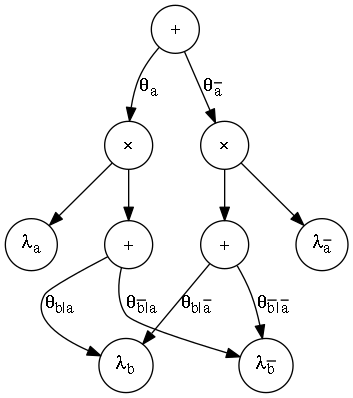
\includegraphics[scale=0.4]{imgs/simple_spn.png}
  \end{figure}
  \begin{equation*}
    f(A,B)=\lambda_a\lambda_b\theta_a\theta_{b|a}+\lambda_{\overline{a}}\lambda_b
    \theta_{\overline{a}}\theta_{b|\overline{a}}+\lambda_a\lambda_{\overline{b}}\theta_a
    \theta_{\overline{b}|a}+\lambda_{\overline{a}}\lambda_{\overline{b}}
    \theta_{\overline{a}}\theta_{\overline{b}|\overline{a}}
  \end{equation*}
\end{frame}

\begin{frame}
  \frametitle{Inferência por Retropropagação}

  \begin{figure}[h]
    \centering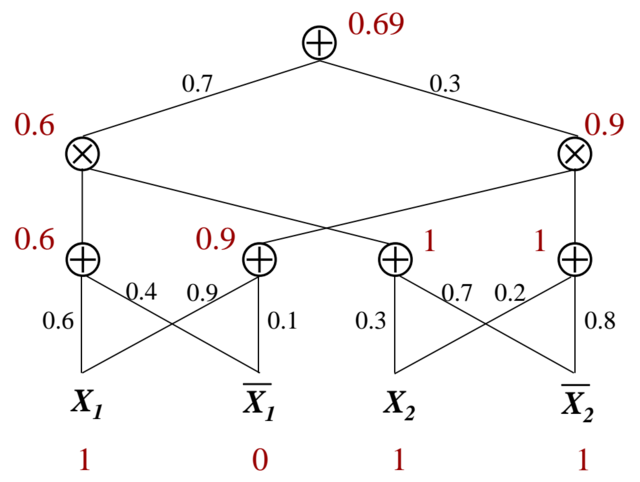
\includegraphics[scale=0.25]{imgs/marginals.png}
  \end{figure}
  \begin{equation*}
    \lambda_{X_1}=1,\lambda_{\overline{X}_1}=0,\lambda_{X_2}=1,\lambda_{\overline{X}_2}=1
  \end{equation*}
  \begin{equation*}
    S=\Pr(X_1=true)=f(x_1)=0.69
  \end{equation*}
\end{frame}

\begin{frame}
  \frametitle{Aprendizado}

  Duas classes de aprendizado:
  \begin{enumerate}
    \item Paramétrico~\cite{poon-domingos}
      \begin{itemize}
        \item Gradiente
        \item EM (expectation-maximization)
      \end{itemize}
    \item Estrutural~\cite{gens-domingos}
  \end{enumerate}
\end{frame}

%--------------------------------------------------------------------------------------------------

\section{Conclusões}

\begin{frame}
  \frametitle{Semelhanças com Redes Neurais}

  \begin{enumerate}
    \item Estrutura
    \item Neurônios
    \item Retropropagação (backpropagation)
    \item RNs de Convolução
    \item Arquitetura profunda
    \item Representa uma função
    \item Mais camadas ocultas, melhor
  \end{enumerate}
\end{frame}

\begin{frame}
  \frametitle{Relação com o Cortex}

  \begin{itemize}
    \item Neurônios piramidais $\equiv$ nós soma
    \item Neurônios estrelados $\equiv$ nós max (produto)
    \item Cortex $\equiv$ SPNs com múltiplas raízes
    \item Raciocínio humano é mais probabilístico do que lógico
  \end{itemize}

  Mais informações no artigo~\cite{poon-domingos}.
\end{frame}

%--------------------------------------------------------------------------------------------------

\section{Planejamento}

\begin{frame}
  \frametitle{Estudo planejado}

  \begin{enumerate}
    \item Base teórica
      \begin{enumerate}
        \item Teoria de Probabilidade
        \item Modelos Probabilísticos Baseados em Grafos
      \end{enumerate}
    \item Inferência em SPNs
      \begin{enumerate}
        \item Função de partição
        \item Marginais
        \item MAP
        \item MPE
      \end{enumerate}
    \item Aprendizado de SPNs
      \begin{enumerate}
        \item Paramétrico
        \item Estrutural
      \end{enumerate}
  \end{enumerate}
\end{frame}

%--------------------------------------------------------------------------------------------------

\section[Referências]{Referências e Bibliografia}
\begin{frame}[t,allowframebreaks]
  \frametitle{Referências e Bibliografia}
  \footnotesize
  \nocite{bayes-net-darwiche}
  \nocite{diff-approach-darwiche}
  \nocite{inference-nphard}
  \nocite{pgm-koller}
  \nocite{pearl-1988}
  \nocite{peharz-spn}
  \printbibliography[]
\end{frame}

\end{document}
